\documentclass[conference]{IEEEtran} % LaTeX2e
\usepackage{amssymb,amsmath,graphicx,float}

\newcommand\real{\mathbb{R}}

\begin{document}

\title{Model Predictive Control of a Mobile Robot Using Linearization}

\author{\authorblockN{Felipe K\"{u}hne}
\authorblockA{Federal University of Rio Grande do Sul\\
Electrical Engineering Department\\
Av. Oswaldo Aranha, 103\\
Porto Alegre, RS 90035-190 Brazil\\
Email: kuhne@eletro.ufrgs.br}
\and
\authorblockN{Walter Fetter Lages}
\authorblockA{Federal University of Rio Grande do Sul\\
Electrical Engineering Department\\
Av. Oswaldo Aranha, 103\\
Porto Alegre, RS 90035-190 Brazil\\
Email: fetter@eletro.ufrgs.br}
\and
\authorblockN{Jo\~{a}o Manoel Gomes da Silva Jr.}
\authorblockA{Federal University of Rio Grande do Sul\\
Electrical Engineering Department\\
Av. Oswaldo Aranha, 103\\
Porto Alegre, RS 90035-190 Brazil\\
Email: jmgomes@eletro.ufrgs.br}
}

\maketitle

\begin{abstract}
This paper presents an optimal control scheme for a wheeled mobile robot (WMR) with nonholonomic constraints. It is well known that a WMR with nonholonomic constraints can not be feedback stabilized through continuously differentiable, time-invariant control laws. By using model predictive control (MPC), a discontinuous control law is naturally obtained. One of the main advantages of MPC is the ability to handle constraints (due to state or input limitations) in a straightforward way. Quadratic programming (QP) is used to solve a linear MPC by successive linearization of an error model of the WMR. Simulation and experimental results are shown.
\end{abstract}
%\begin{keywords}
%Wheeled mobile robots, model predictive control, trajectory tracking.
%\end{keywords}
%\thispagestyle{empty}\pagestyle{empty}

\section{Introduction}
\label{sec:intro}

The field of mobile robot control has been the focus of great research effort in the past decades. Besides the apparent simplicity of the kinematic model of a wheeled mobile robot (WMR), the existence of nonholonomic (non-integrable) constraints turns the design of stabilizing control laws for those systems in a considerable challenge. Due to Brockett
conditions~\cite{brockett82}, a continuously differentiable, time-invariant stabilizing feedback control law can not be obtained. To overcome these limitations most works uses discontinuous (non-smooth) and time-variant control laws~\cite{bloch89,samson91,canudas92,yamamoto94,murray97}. Recent works dealing with robust and adaptive control of WMRs can be found in \cite{oya03,dixon04}.

However, in realistic implementations it is difficult to obtain good performance, due to the constraints on inputs or states that naturally arise. None of the previously cited authors have taken those constraints into account. This can be done in a straightforward way by using model predictive control (MPC) schemes. For a WMR this is an important advantage,
since the position of the robot can be restricted to belong to a secure region of operation. By considering input limitations, control actions that stay within actuators saturation limit can be generated.

Model Predictive Control is a control strategy that uses the model of the system to obtain an optimal control sequence by minimizing an objective function. At each sample interval, the model provides a prediction of process states over a prediction horizon. Based on that, an objective function is optimized with respect to the future open-loop control system
inputs. Although prediction and optimization are computed over a future horizon, only the values of the inputs for the current sampling interval are used and the same procedure is repeated at the next sampling time. This mechanism is known as {\it moving} or {\it receding horizon} strategy, in reference to the way in which the time window shifts forward from one time step to the next.

For complex constrained multivariable control problems, MPC has become the accepted standard in the process industries~\cite{bemporad02}. It is used in many cases, where plants being controlled are sufficiently {\em slow} to allow its implementation~\cite{mayne98}. However, for systems with fast and/or nonlinear dynamics, like the WMRs, the implementation of such technique remains fundamentally limited in applicability, due to large amount of {\em on-line} computation required \cite{cannon00}. In this paper we overcome this problem by using a successive-linearization approach, where a linear MPC is solved by quadratic programming (QP) problem. It is shown that even a real-time implementation is possible. Although MPC is not a new control method, works dealing with MPC of WMRs are recent and sparse~\cite{ollero91,rico99,essen01}.

The remainder of this paper is organized as follows: in the next section the kinematic model of the WMR is shown. The MPC algorithm is depicted in section~\ref{sec:mpc}. Simulation results in {\sc Matlab} are shown in section~\ref{sec:simulations}, where an eight-like trajectory is used as reference. Section~\ref{sec:exp} presents some real-time implementation details.


\section{Kinematic Model of the WMR}
\label{sec:model}

In this section the kinematic model of the WMR is described. A mobile robot
made up of a rigid body and non deforming wheels is considered (see Fig.~\ref{fig:robot}). It is assumed that the vehicle moves without slipping on a plane. The kinematics of the WMR is given by:

\begin{equation}
\label{eqn:model}
	\left\{
		\begin{aligned}
			\dot x	  &= v\cos\theta \\
			\dot y	  &= v\sin\theta \\
			\dot \theta &= w
		\end{aligned}
	\right.
\end{equation}

\noindent where ${\bf x}\triangleq[x~~y~~\theta]^T$ describes the configuration (position and orientation) of the center of the active wheels' axle, $C$, with respect to a global inertial frame $\{O,X,Y\}$. ${\bf u}\triangleq[v~~w]^T$ are the manipulated (control) variable, where $v$ and $w$ are the linear and the angular velocities, respectively.

\begin{figure}[htbp]
\begin{center}
    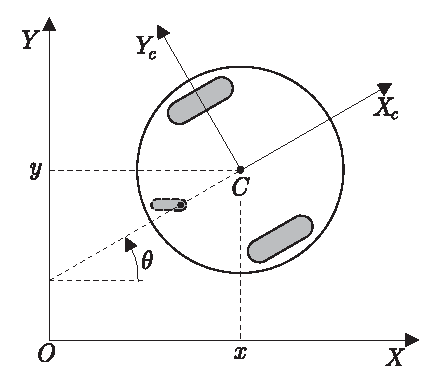
\includegraphics[width=0.67\linewidth]{Figures/robot.eps}
    \caption{Coordinate system of the WMR.}
    \label{fig:robot}
\end{center}
\end{figure}

By using the Euler method to discretize (\ref{eqn:model}):

\begin{equation*}
	\dot{\bf x} \approx \frac{{\bf x}(k+1)-{\bf x}(k)}{T},
\end{equation*}

\noindent where $T$ is the sampling period and $k$ is the time step, we have the following nonlinear, discrete-time model:

\begin{equation}
\label{eqn:discretemodel}
	\left\{
		\begin{aligned}
			x(k+1)	    &= x(k) + v(k)\cos\theta(k)T \\
			y(k+1)	    &= y(k) + v(k)\sin\theta(k)T \\
			\theta(k+1) &= \theta(k) + w(k)T \\
		\end{aligned}
	\right.
\end{equation} 

\subsection{Derivation of a Linear Error Model}

To obtain a linear model, an error model with respect to a reference trajectory $({\bf x}_r,{\bf u}_r)$ is considered. This can be done by expanding (\ref{eqn:discretemodel}) in Taylor series around the reference trajectory. The resulting error will be used in Section \ref{sec:mpc} for the solution of a linear MPC problem.

The model (\ref{eqn:discretemodel}) has the form ${\bf x}(k+1)=f({\bf x}(k),{\bf u}(k))$. Expanding in Taylor series around the point $({\bf x}_r(k),{\bf u}_r(k))$ and neglecting higher order terms the following expression is obtained:

\begin{equation}
\begin{split}
\label{eq:taylor}
	f({\bf x}(k),{\bf u}(k)) \approx f({\bf x}_r(k),{\bf u}_r(k)) + \\ + \left.\frac{\partial f({\bf x}(k),{\bf u}(k))}{\partial{\bf x}(k)}\right|_{\begin{smallmatrix}{\bf x}(k)={\bf x}_r(k) \\ {\bf u}(k)={\bf u}_r(k) \end{smallmatrix}}({\bf x}(k)-{\bf x}_r(k)) + \\ + \left.\frac{\partial f({\bf x}(k),{\bf u}(k))}{\partial{\bf u}(k)}\right|_{\begin{smallmatrix}{\bf x}(k)={\bf x}_r(k) \\ {\bf u}(k)={\bf u}_r(k) \end{smallmatrix}}({\bf u}(k)-{\bf u}_r(k))
\end{split}
\end{equation}

By considering a reference car described by ${\bf x}_r(k+1)=f({\bf x}_r(k),{\bf u}_r(k))$, it follows from (\ref{eq:taylor}) that

\begin{equation}\label{eqn:error}
	\tilde{\bf x}(k+1) = {\bf A}(k)\tilde{\bf x}(k)+{\bf B}(k)\tilde{\bf u}(k),
\end{equation}
\noindent where
\begin{equation*}
	\tilde{\bf x}(k) \triangleq \begin{bmatrix}
		\cos\theta_r(k)  & \sin\theta_r(k) & 0 \\
		-\sin\theta_r(k) & \cos\theta_r(k) & 0 \\
		0		       & 0		     & 1
	\end{bmatrix} 
	\begin{bmatrix}
		x(k)-x_r(k) \\ y(k)-y_r(k) \\ \theta(k)-\theta_r(k)
	\end{bmatrix},
\end{equation*}
$$
\tilde{\bf u}(k)\triangleq{\bf u}(k)-{\bf u}_r(k)
$$
\noindent and
\begin{align*}
	{\bf A}(k) &= \begin{bmatrix}
		1 & 0 & -v_r(k)\sin\theta_r(k)T \\
		0 & 1 &  v_r(k)\cos\theta_r(k)T \\
		0 & 0 & 1
	\end{bmatrix} \\
	{\bf B}(k) &= \begin{bmatrix}
		\cos\theta_r(k)T & 0 \\
		\sin\theta_r(k)T & 0 \\
		0 			  & T
	\end{bmatrix}
\end{align*}

Indeed, the convergence of ${\bf x}$ to ${\bf x}_r$ is equivalent to the convergence of $\tilde{\bf x}$ to the set ${\cal O}=\{{\bf x}|(\tilde x,\tilde y,\tilde\theta)=(0,0,2\pi n)\},n\in \{0,\pm1,\pm2,\ldots\}$.

In~\cite{bloch89} it is shown that the nonlinear, nonholonomic system (\ref{eqn:model}) is fully controllable, i.e., it can be steered from any initial state to any final state in finite time by using finite inputs. It is easy to see that when the robot is not moving, the linearization about a stationary operating point is not controllable. However, this linearization becomes controllable as long as the control input ${\bf u}$ is not zero~\cite{samson91}. This implies the tracking of a reference trajectory being possible with linear MPC~\cite{essen01}.


\section{The MPC Algorithm}
\label{sec:mpc}

It was said in section~\ref{sec:intro} that the essence of a MPC scheme is to optimize predictions of process behavior over the control inputs. Such prediction is accomplished by using a process model over a finite time interval, called the {\em prediction horizon}. At each sampling time, the model predictive controller generates an optimal control sequence by solving a optimization problem. The first element of this sequence is applied to the plant. The problem is solved again at the next sampling time using the updated process measurements and a shifted horizon.

For the sake of simplicity, we assume in this work that the states of the plant are always available for measurement and that there are no plant/model mismatch. Also, in order to design the linear controller, it is assumed that the pair $({\bf A}(k),{\bf B}(k))$ is always (at any $k$) stabilizable.

To the problem concerned here, the cost function to be minimized can be stated as a quadratic function of the states and control inputs:
\begin{multline}\label{eqn:cost}
	\Phi(k) = \sum_{j=1}^{N}\tilde{\bf x}^T(k+j|k){\bf Q}\tilde{\bf x}(k+j|k) + \\ + \tilde{\bf u}^T(k+j-1|k){\bf R}\tilde{\bf u}(k+j-1|k),
\end{multline}
\noindent where $N$ is the prediction horizon and ${\bf Q}$, ${\bf R}$ are weighting matrices, with ${\bf Q}\geq 0$ and ${\bf R}>0$. The notation $a(m|n)$ indicates the value of $a$ at the instant $m$ predicted at instant $n$.

Hence, the optimization problem can be stated as to find $\tilde{\bf u}^\star$ such that:
\begin{equation*}
	\tilde{\bf u}^\star = \arg\min_{\tilde{\bf u}}\left\{\Phi(k)\right\}
\end{equation*}
\noindent s. a.
\begin{equation*}
	\tilde{\bf u}_{min} \leq \tilde{\bf u} \leq \tilde{\bf u}_{max}
\end{equation*}

\noindent where $\Phi(k)$ is the {\em cost function}, $\tilde{\bf u}$ is the
free variable in the optimization, and $\tilde{\bf u}_{min}$ and
$\tilde{\bf u}_{max}$ are its inferior and superior limits, respectively.

The problem of minimizing (\ref{eqn:cost}) is solved at each time step $k$, yelding a sequence of minimizers $\{\tilde{\bf u}^\star(k|k),\cdots,\tilde{\bf u}^\star(k+N-1|k)\}$ and the optimal cost $\Phi^\star(k)$. The MPC control law is implicitly given by the first control action of the sequence of minimizers, $\tilde{\bf u}^\star(k|k)$. A block diagram with all components of the system is shown in Fig. \ref{fig:bloco}.

\begin{figure}[htbp]
\begin{center}
    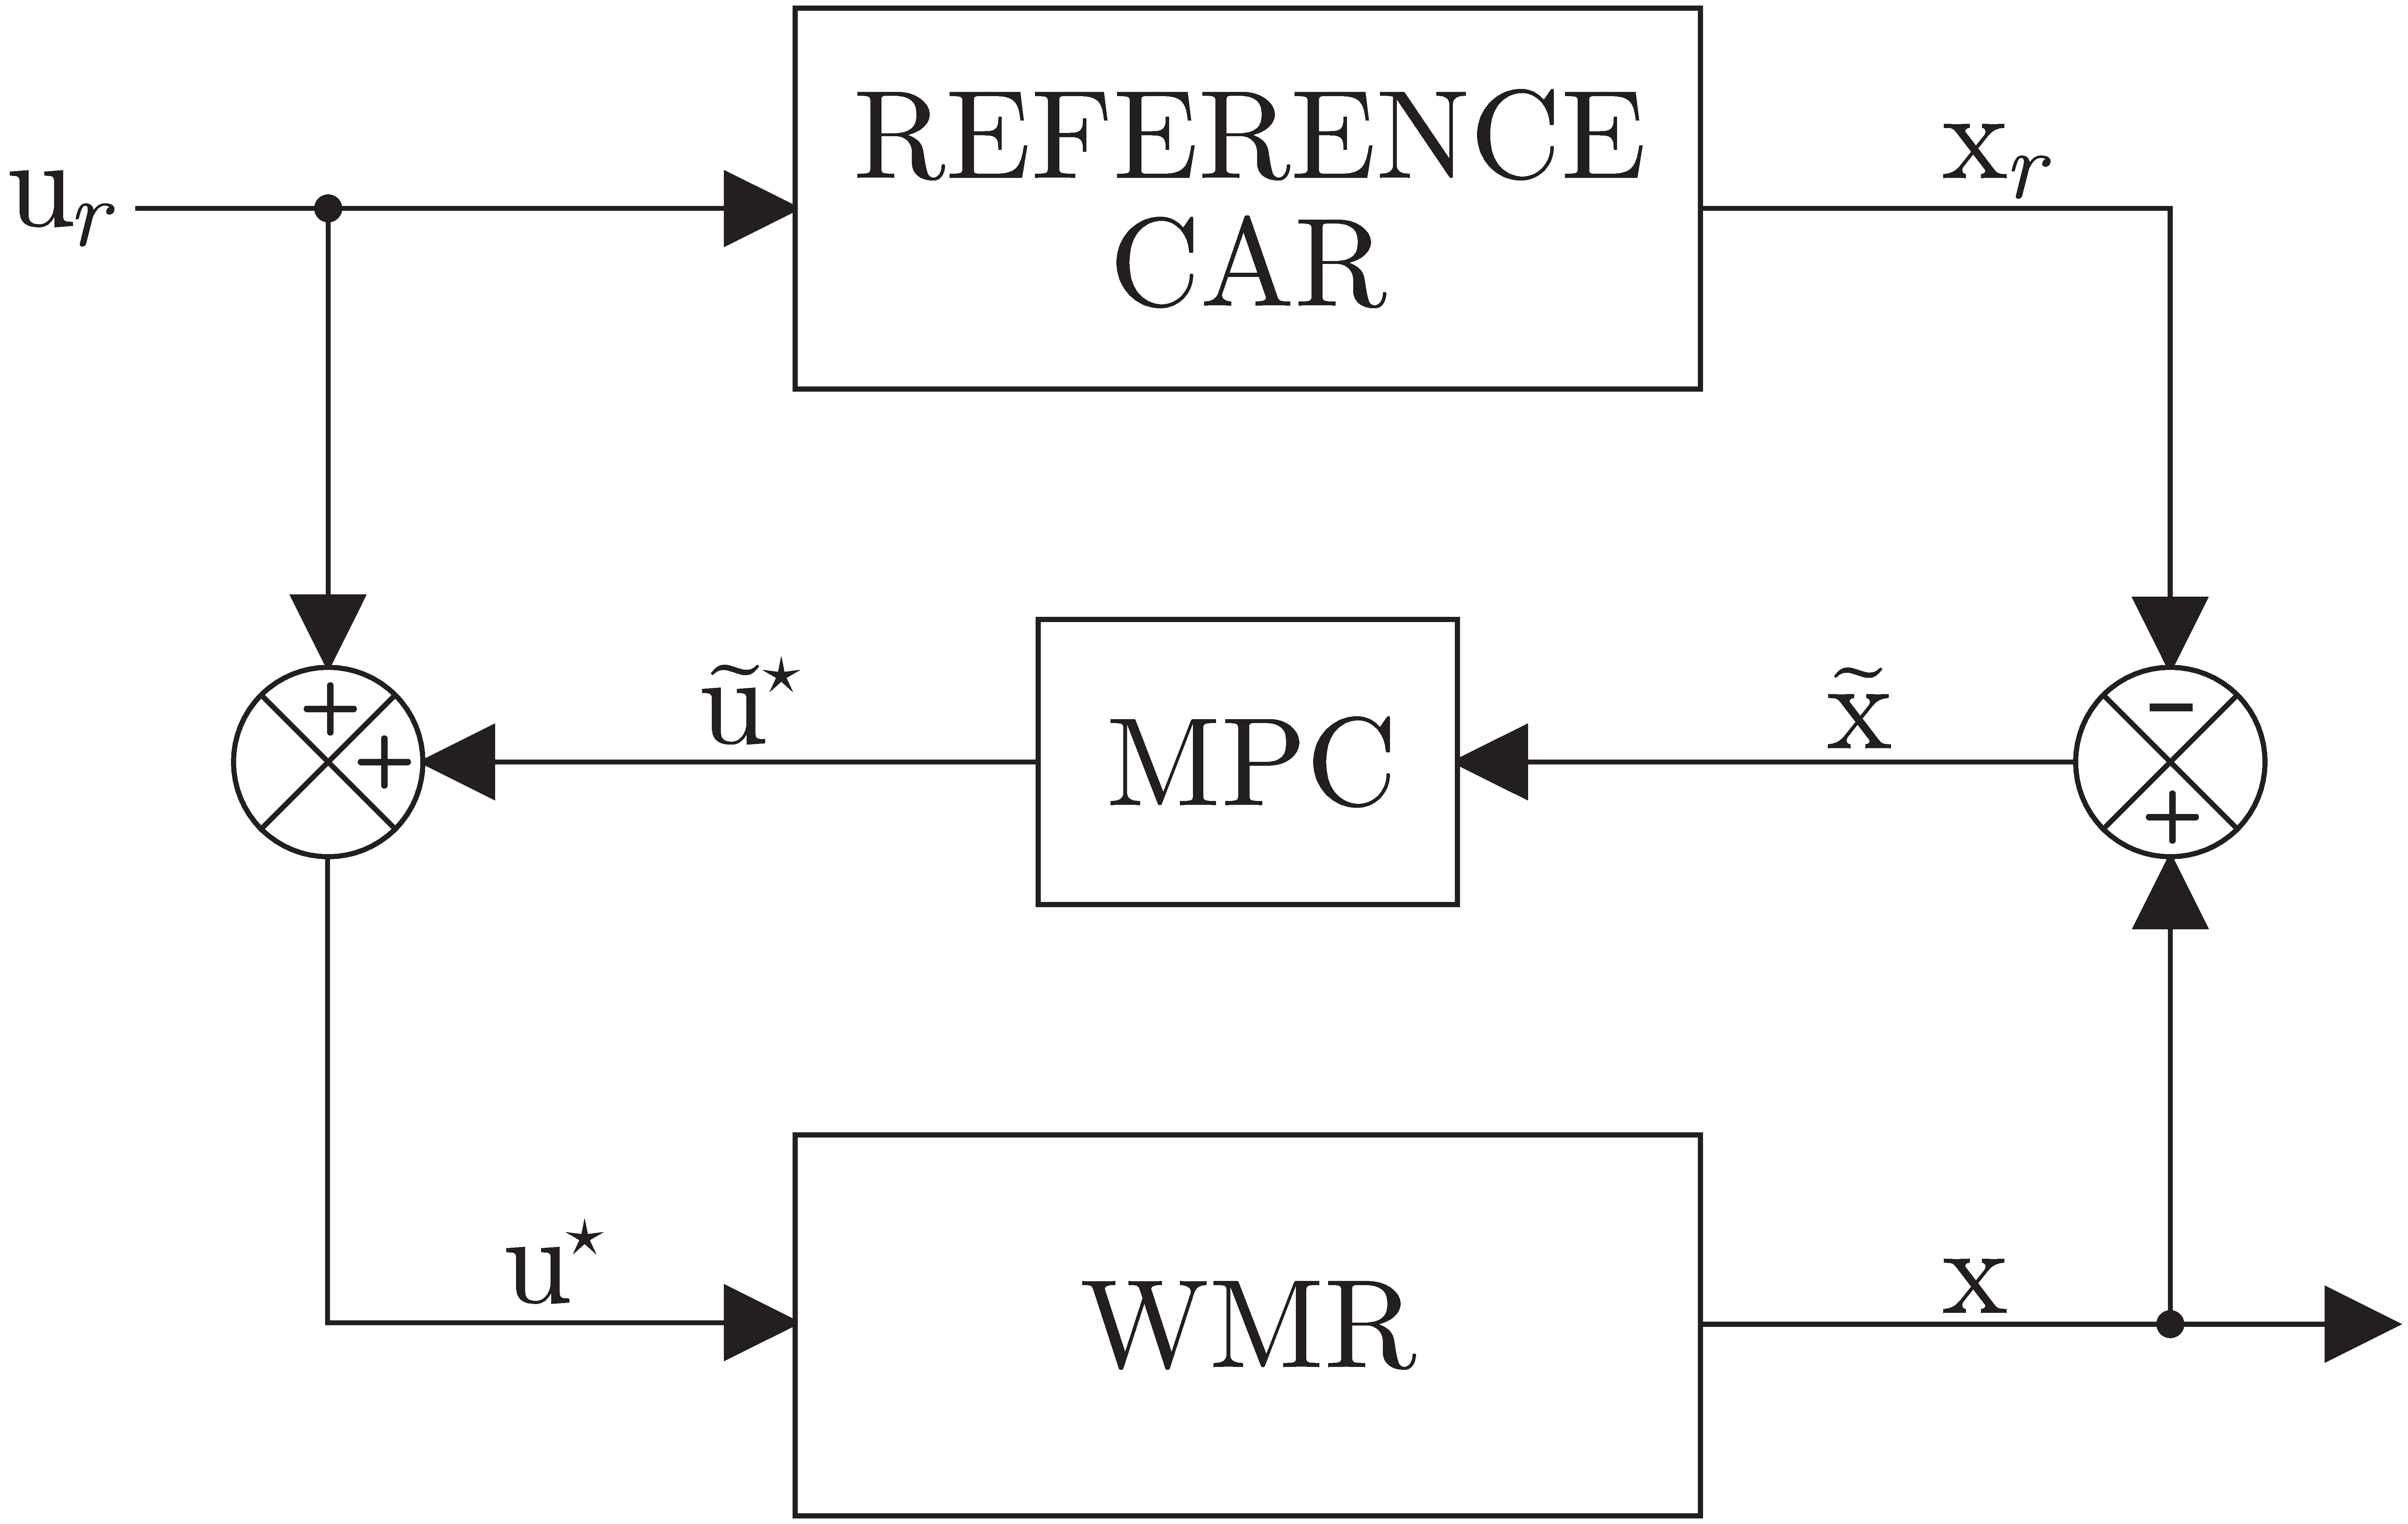
\includegraphics[width=.84\linewidth]{Figures/bloco.eps}
    \caption{Block diagram of the system.}
    \label{fig:bloco}
\end{center}
\end{figure}

\subsection{Derivation of the Quadratic Programming Problem}
\label{sec:qp}

To put the optimization problem in a usual QP formulation, we introduce the stacked vectors
\begin{equation*}
	\bar{\bf x}(k) \triangleq \begin{bmatrix}
		\tilde{\bf x}(k+1|k) \\ \tilde{\bf x}(k+2|k) \\ \vdots \\ \tilde{\bf x}(k+N|k) 
	\end{bmatrix} \quad
	\bar{\bf u}(k) \triangleq \begin{bmatrix}
		\tilde{\bf u}(k|k)  \\ \tilde{\bf u}(k+1|k) \\ \vdots \\ \tilde{\bf u}(k+N-1|k)
	\end{bmatrix}
\end{equation*}

Thus, equation (\ref{eqn:cost}) can be rewritten as:
\begin{equation}\label{eqn:cost2}
	\Phi(k) = \bar{\bf x}^T(k)\bar{\bf Q}\bar{\bf x}(k) + \bar{\bf u}^T(k)\bar{\bf R}\bar{\bf u}(k),
\end{equation}
with
\begin{equation*}
	\bar {\bf Q} \triangleq \begin{bmatrix}
		{\bf Q} & {\bf 0} & \cdots & {\bf 0} \\
		{\bf 0} & {\bf Q} & \cdots & {\bf 0} \\
		\vdots  & \vdots  & \ddots & \vdots  \\
		{\bf 0} & {\bf 0} & \cdots & {\bf Q}
	\end{bmatrix} \quad
	\bar {\bf R} \triangleq \begin{bmatrix}
		{\bf R} & {\bf 0} & \cdots & {\bf 0} \\
		{\bf 0} & {\bf R} & \cdots & {\bf 0} \\
		\vdots  & \vdots  & \ddots & \vdots  \\
		{\bf 0} & {\bf 0} & \cdots & {\bf R}
	\end{bmatrix}
\end{equation*}

With the above definitions, it is possible to rewrite $\bar{\bf x}(k)$ as:
\begin{equation}\label{eqn:exbar}
	\bar{\bf x}(k) = \bar{\bf A}(k)\tilde{\bf x}(k|k)+{\bf S}(k)\bar{\bf u}(k),
\end{equation}
with
\begin{equation*}
	\bar{\bf A}(k) \triangleq \begin{bmatrix}
		{\bf A}(k|k) \\ {\bf A}(k|k){\bf A}(k+1|k) \\ \vdots \\ \alpha(k,0)
	\end{bmatrix}
\end{equation*}
{\small
\begin{multline*}
		{\bf S}(k) \triangleq \\ \begin{bmatrix}
			{\bf B}(k|k)		       & {\bf 0} 			    	 & \cdots & {\bf 0}         \\
			{\bf A}(k+1|k){\bf B}(k|k) & {\bf B}(k+1|k)      	 & \cdots & {\bf 0}         \\
			\vdots			       & \vdots				 & \ddots & \vdots          \\
			\alpha(k,1){\bf B}(k|k)    & \alpha(k,2){\bf B}(k+1|k) & \cdots & {\bf B}(k+N-1|k)
		\end{bmatrix}
\end{multline*}
}
where the operator $\alpha(k,j)$ is defined as:
\begin{equation*}
	\alpha(k,j) \triangleq \prod_{i=j}^{N-1}{\bf A}(k+i|k),
\end{equation*}

With (\ref{eqn:cost2}) and (\ref{eqn:exbar}) at hands, and after some algebraic manipulations, we can rewrite the cost function (\ref{eqn:cost}) in a standard quadratic form:
\begin{equation}
	\Phi(k) = \frac{1}{2}\bar{\bf u}^T(k){\bf H}(k)\bar{\bf u}(k) + {\bf f}^T(k)\bar{\bf u}(k) + {\bf d}(k)
\end{equation}

%To put the optimization problem in a usual QP formulation, we introduce the stacked vectors
%\begin{equation*}
%	{\bar{\tilde{\bf x}}}(k) \triangleq \begin{bmatrix}
%		\tilde{\bf x}(k+1|k) \\ \tilde{\bf x}(k+2|k) \\ \vdots \\ \tilde{\bf x}(k+N|k) 
%	\end{bmatrix} \quad
%	{\bar{\tilde{\bf u}}}(k) \triangleq \begin{bmatrix}
%		\tilde{\bf u}(k|k)  \\ \tilde{\bf u}(k+1|k) \\ \vdots \\ \tilde{\bf u}(k+N-1|k)
%	\end{bmatrix}
%\end{equation*}
%
%Thus, equation (\ref{eqn:cost}) can be rewritten as:
%\begin{equation}\label{eqn:cost2}
%	\Phi(k) = {\bar{\tilde{\bf x}}}^T(k)\bar{\bf Q}{\bar{\tilde{\bf x}}}(k) + {\bar{\tilde{\bf u}}}^T(k)\bar{\bf R}{\bar{\tilde{\bf u}}}(k),
%\end{equation}
%with
%\begin{equation*}
%	\bar {\bf Q} \triangleq \begin{bmatrix}
%		{\bf Q} & {\bf 0} & \cdots & {\bf 0} \\
%		{\bf 0} & {\bf Q} & \cdots & {\bf 0} \\
%		\vdots  & \vdots  & \ddots & \vdots  \\
%		{\bf 0} & {\bf 0} & \cdots & {\bf Q}
%	\end{bmatrix} \quad
%	\bar {\bf R} \triangleq \begin{bmatrix}
%		{\bf R} & {\bf 0} & \cdots & {\bf 0} \\
%		{\bf 0} & {\bf R} & \cdots & {\bf 0} \\
%		\vdots  & \vdots  & \ddots & \vdots  \\
%		{\bf 0} & {\bf 0} & \cdots & {\bf R}
%	\end{bmatrix}
%\end{equation*}
%
%With the above definitions, it is possible to rewrite $\bar{\tilde{\bf x}}$ as:
%\begin{equation}\label{eqn:exbar}
%	{\bar{\tilde{\bf x}}}(k) = \bar{\bf A}(k)\tilde{\bf x}(k|k)+{\bf S}(k){\bar{\tilde{\bf u}}}(k),
%\end{equation}
%with
%\begin{equation*}
%	\bar{\bf A}(k) \triangleq \begin{bmatrix}
%		{\bf A}(k|k) \\ {\bf A}(k|k){\bf A}(k+1|k) \\ \vdots \\ \alpha(k,0)
%	\end{bmatrix}
%\end{equation*}
%{\small
%\begin{multline*}
%		{\bf S}(k) \triangleq \\ \begin{bmatrix}
%			{\bf B}(k|k)		       & {\bf 0} 			    	 & \cdots & {\bf 0}         \\
%			{\bf A}(k+1|k){\bf B}(k|k) & {\bf B}(k+1|k)      	 & \cdots & {\bf 0}         \\
%			\vdots			       & \vdots				 & \ddots & \vdots          \\
%			\alpha(k,1){\bf B}(k|k)    & \alpha(k,2){\bf B}(k+1|k) & \cdots & {\bf B}(k+N-1|k)
%		\end{bmatrix}
%\end{multline*}
%}
%where 
%\begin{equation*}
%	\alpha(k,j) \triangleq \prod_{i=j}^{N-1}{\bf A}(k+i|k),
%\end{equation*}
%
%With (\ref{eqn:cost2}) and (\ref{eqn:exbar}) at hands, and after some algebraic manipulations, we can rewrite the cost function (\ref{eqn:cost}) in a standard quadratic form:
%\begin{equation}
%	\Phi(k) = \frac{1}{2}{\bar{\tilde{\bf u}}}^T(k){\bf H}(k){\bar{\tilde{\bf u}}}(k) + {\bf f}^T(k){\bar{\tilde{\bf u}}}(k) + {\bf d}(k)
%\end{equation}
with
\begin{align*}
	{\bf H}(k) &\triangleq 2\left({\bf S}^T(k)\bar{\bf Q}{\bf S}(k)+\bar{\bf R}\right) \\
	{\bf f}(k) &\triangleq 2{\bf S}^T(k)\bar{\bf Q}\bar{\bf A}(k)\tilde{\bf x}(k|k) \\
	{\bf d}(k) &\triangleq \tilde{\bf x}^T(k|k)\bar{\bf A}^T(k)\bar{\bf Q}\bar{\bf A}(k)\tilde{\bf x}(k|k)
\end{align*}

The matrix ${\bf H}$ is a {\em Hessian} matrix, and must be positive definite. It describes the quadratic part of the cost function, and the vector ${\bf f}$ describes the linear part. $\bf d$ is independent of $\tilde{\bf u}$ and hence vanishes of the optimization problem.

For the sake of simplicity and to give a major focus on the optimization problem, it is considered here the inexistence of plant/model mismatch. However, there are some inherent features to eletro-mechanical systems that must be taken into account in control problems like the one treated here. In this case, as the wheels are driven by elecrical motors, these features are the actuators' saturations. With MPC, this can be done in a straightforward way by defining upper and lower bounds on the amplitude of the control action. The optimization problem must then be solved guaranteeing that the control will remain between these bounds. Hence, the following control constraint can be written:

\begin{equation}\label{eqn:uconstr}
	{\bf u}_{min}(k) \leq {\bf u}(k) \leq {\bf u}_{max}(k),
\end{equation}
with the lower and upper bounds 
\begin{equation*}
	{\bf u}_{min}(k) = \begin{bmatrix}
		v_{min}(k) \\ w_{min}(k)
	\end{bmatrix} \quad 
	{\bf u}_{max}(k) = \begin{bmatrix}
		v_{max}(k) \\ w_{max}(k)
	\end{bmatrix}
\end{equation*}

In this case, as the free variable in the optimization is the vector $\bar{\bf u}(k)$, the constraint (\ref{eqn:uconstr}) must be rewritten with respect to this variable (notice again that $\tilde{\bf u}(k)={\bf u}(k)-{\bf u}_r(k)$):
\begin{equation*}
	{\bf u}_{min}(k) - {\bf u}_r(k) \leq \tilde{\bf u}(k) \leq {\bf u}_{max}(k) - {\bf u}_r(k),
\end{equation*}
or, in the stacked way,
\begin{equation*}
	\bar{\bf u}_{min}(k) - \bar{\bf u}_r(k) \leq \bar{\bf u}(k) \leq \bar{\bf u}_{max}(k) - \bar{\bf u}_r(k)
\end{equation*}
\noindent with
\begin{align*}
	\bar{\bf u}_{min}(k) &\triangleq \begin{bmatrix}
		{\bf u}_{min}(k) \\ {\bf u}_{min}(k+1) \\ \vdots \\ {\bf u}_{min}(k+N-1)
	\end{bmatrix} \\
	\bar{\bf u}_{max}(k) &\triangleq \begin{bmatrix}
		{\bf u}_{max}(k) \\ {\bf u}_{max}(k+1) \\ \vdots \\ {\bf u}_{max}(k+N-1)
	\end{bmatrix} \\
	\bar{\bf u}_r(k) &\triangleq \begin{bmatrix}
		{\bf u}_r(k) \\ {\bf u}_r(k+1) \\ \vdots \\ {\bf u}_r(k+N-1)
	\end{bmatrix}
\end{align*}

%Now it is possible to define constraints, for example, in the amplitude of the control action ${\bf u}(k)$ or, in the stacked form, $\bar {\bf u}(k)\triangleq[{\bf u}^T(k|k)~~\cdots~~{\bf u}^T(k+N-1|k)]^T$. So, we have the following constraint:
%
%\begin{equation}\label{eqn:uconstr}
%	\bar{\bf u}_{min}(k) \leq \bar{\bf u}(k) \leq \bar{\bf u}_{max}(k),
%\end{equation}
%with the limits 
%\begin{equation*}
%	{\bf u}_{min}(k) = \begin{bmatrix}
%		v_{min}(k) \\ w_{min}(k)
%	\end{bmatrix} \quad 
%	{\bf u}_{max}(k) = \begin{bmatrix}
%		v_{max}(k) \\ w_{max}(k)
%	\end{bmatrix}
%\end{equation*}
%\noindent and
%\begin{align*}
%	\bar{\bf u}_{min}(k) &\triangleq \begin{bmatrix}
%		{\bf u}_{min}(k) \\ {\bf u}_{min}(k+1) \\ \vdots \\ {\bf u}_{min}(k+N-1)
%	\end{bmatrix} \\
%	\bar{\bf u}_{max}(k) &\triangleq \begin{bmatrix}
%		{\bf u}_{max}(k) \\ {\bf u}_{max}(k+1) \\ \vdots \\ {\bf u}_{max}(k+N-1)
%	\end{bmatrix}
%\end{align*}
%
%In this case, the free variable in the optimization is the vector ${\bar{\tilde{\bf u}}}(k)$, and the constraint (\ref{eqn:uconstr}) must be rewritten with respect to this variable (remembering that $\tilde{\bf u}(k)={\bf u}(k)-{\bf u}_r(k)$):
%
%\begin{equation*}
%	\bar{\bf u}_{min}(k) - \bar{\bf u}_r(k) \leq {\bar{\tilde{\bf u}}}(k) \leq \bar{\bf u}_{max}(k) - \bar{\bf u}_r(k)
%\end{equation*}
%where
%\begin{equation*}
%	\bar{\bf u}_r(k) \triangleq \begin{bmatrix}
%		{\bf u}_r(k) \\ {\bf u}_r(k+1) \\ \vdots \\ {\bf u}_r(k+N-1)
%	\end{bmatrix}
%\end{equation*}


\section{Simulation results}
\label{sec:simulations}

In this section, simulation results are shown for the MPC applied to the WMR. The optimization problem has been solved with the {\sc Matlab} routine {\tt quadprog}. The initial configuration of the WMR were: ${\bf x}(0)=[-0.8~~1~~3\pi/2]^T$, ${\bf Q}=diag(1,1,0.5)$, ${\bf R}=0.5{\bf I}_{2\times 2}$ and $N=3$. Constraints in
the amplitude of the control variables were: $v_{min}=0.2 m/s$, $v_{max}=0.4 m/s$, $w_{min}=-0.4 rad/s$ and $w_{max}=0.4 rad/s$. It can be seen that the state converges to the references. In Fig. \ref{fig:traj8} and \ref{fig:states}, the dash-dotted line stands for the reference trajectory of the states.

\begin{figure}[H]\begin{center}
    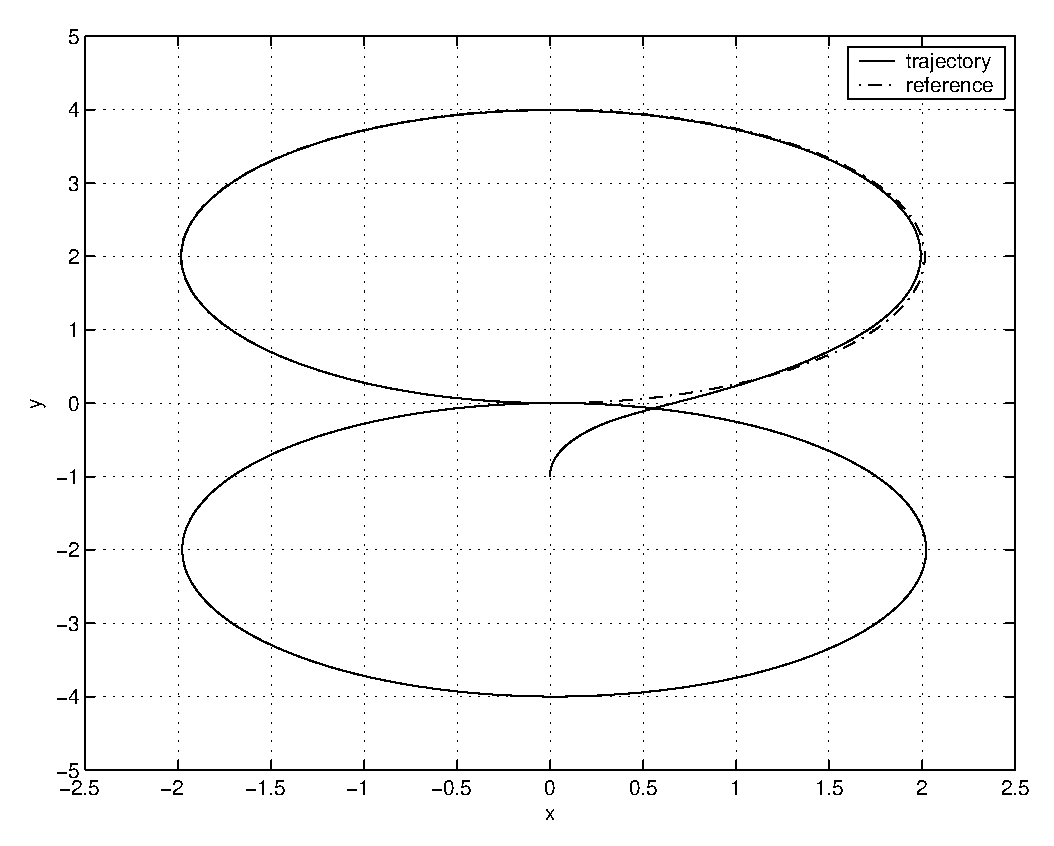
\includegraphics[width=.99\linewidth]{Figures/traj8.eps}
    \caption{Trajectory in the $XY$ plane.}
    \label{fig:traj8}
\end{center}\end{figure}
\begin{figure}[H]\begin{center}
    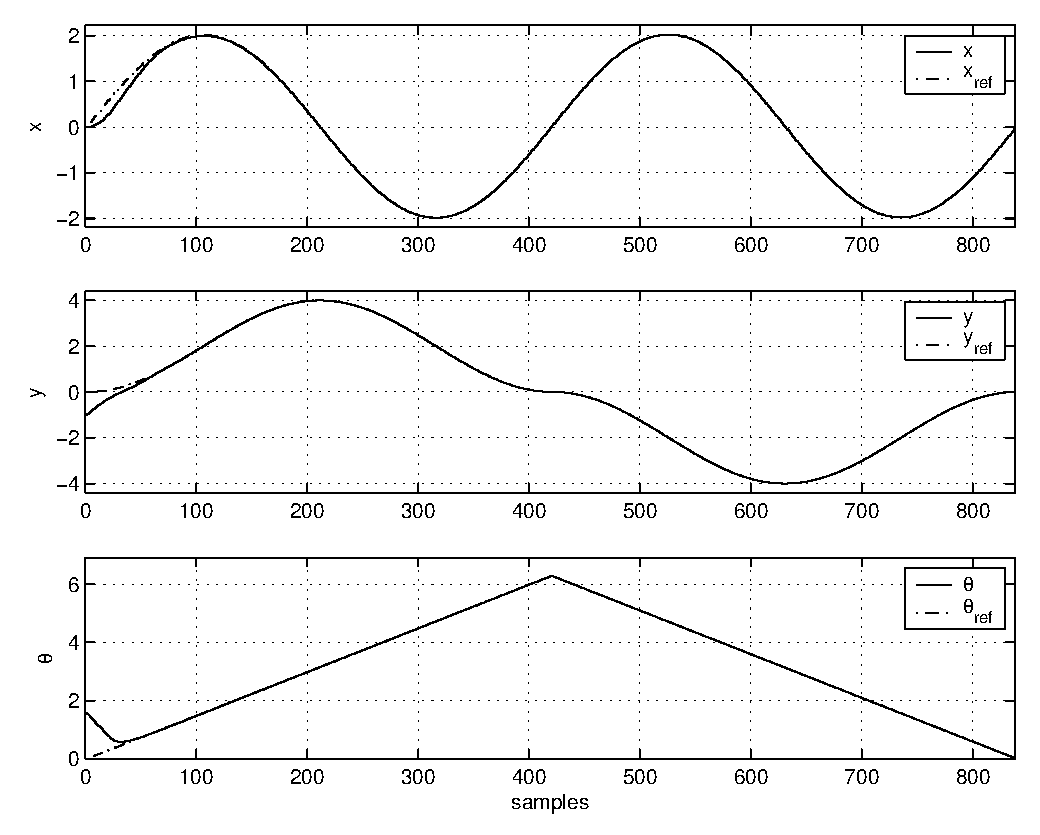
\includegraphics[width=.99\linewidth]{Figures/states.eps}
    \caption{States $x$, $y$ and $\theta$.}
    \label{fig:states}
\end{center}\end{figure}

Figure~\ref{fig:errors} shows the errors of the states converging to zero. In Fig.~\ref{fig:controls}, it can be clearly seen that the control inputs obey the limits imposed by the constraints. As the state and control errors converge to zero (Fig. \ref{fig:errors}), one could say that the value of the cost function must converges to zero too. This fact can be observed in Fig.~\ref{fig:cost}.

\begin{figure}\begin{center}
    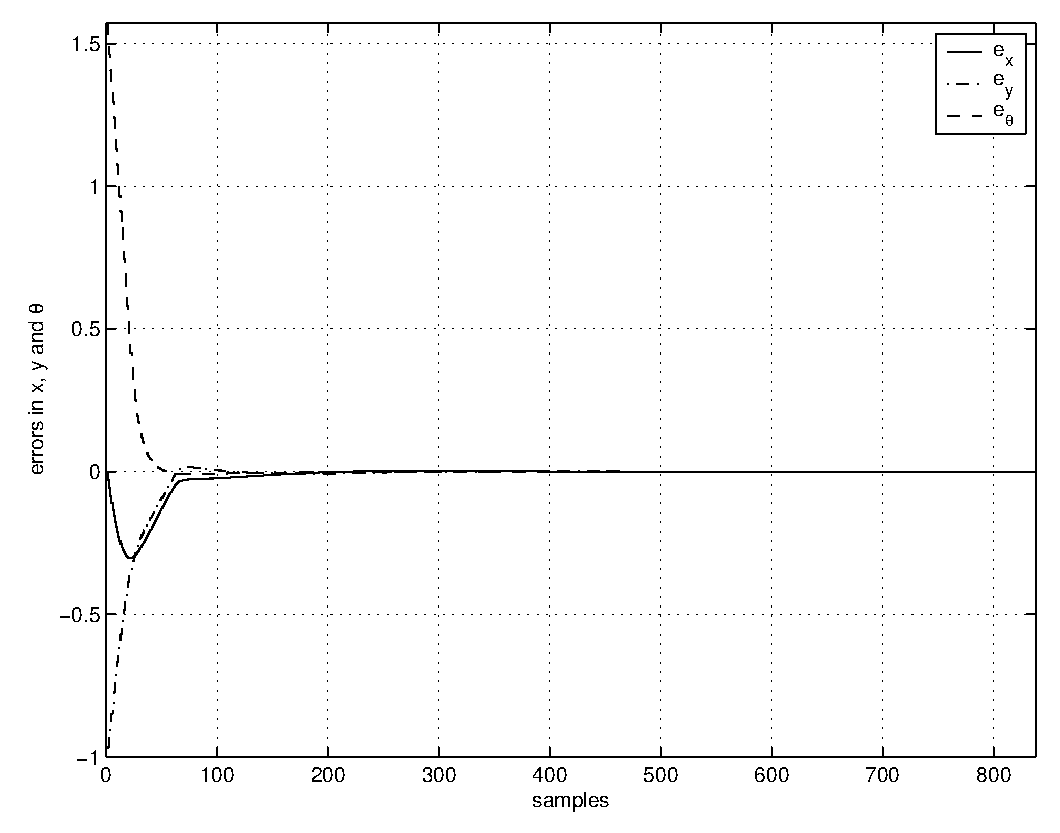
\includegraphics[width=.99\linewidth]{Figures/errors.eps}
    \caption{Errors.}
    \label{fig:errors}
\end{center}\end{figure}
\begin{figure}\begin{center}
    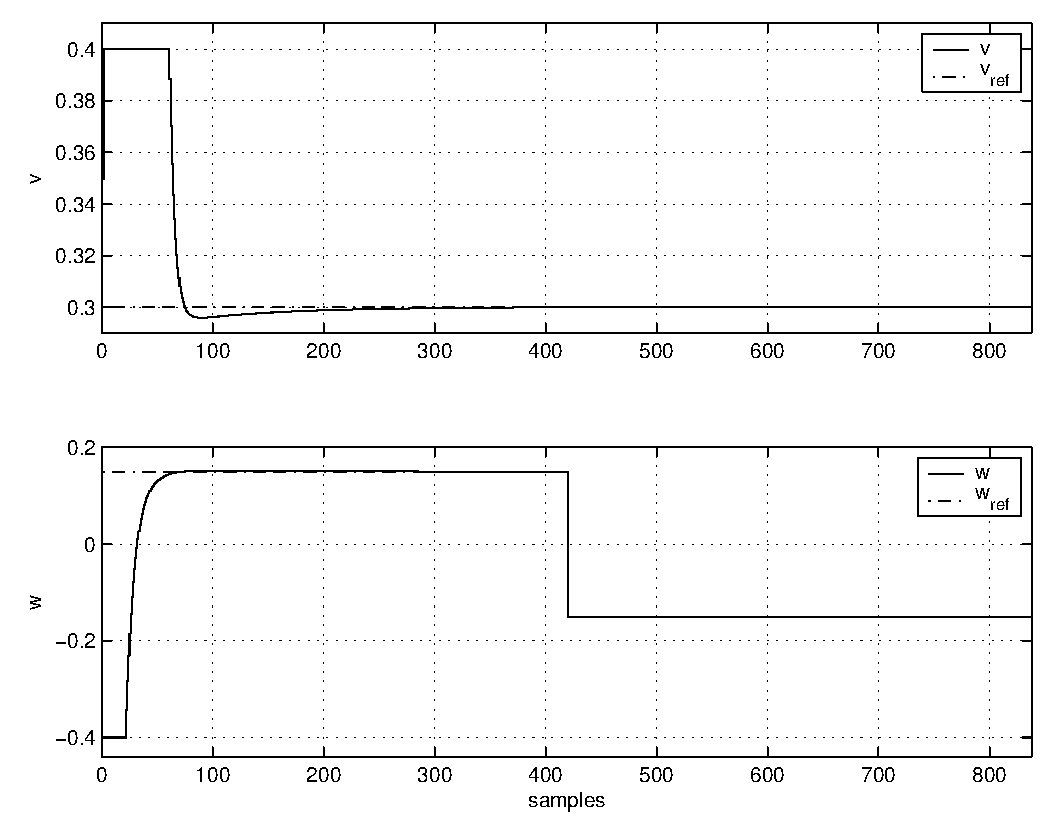
\includegraphics[width=.99\linewidth]{Figures/controls.eps}
    \caption{Controls bounded by the constraints (dotted lines for unconstrained case).}
    \label{fig:controls}
\end{center}\end{figure}
\begin{figure}[H]\begin{center}
    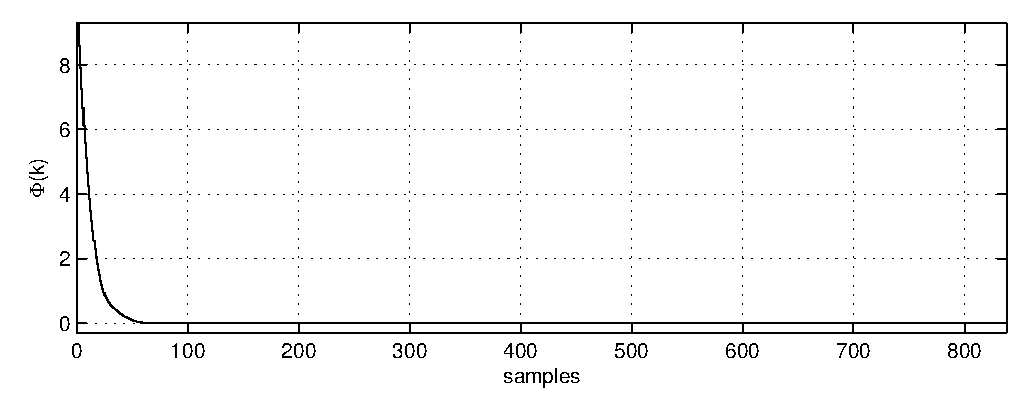
\includegraphics[width=.99\linewidth]{Figures/cost.eps}
    \caption{Cost function $\Phi(k)$.}
    \label{fig:cost}
\end{center}\end{figure}


\section{Experimental Results}
\label{sec:exp}

Fig.~\ref{fig:twil} shows the mobile robot developed in our labs and used in this work. It has a cylindrical geometry with 1.35m in height and 0.30 cm in radius and uses a differential-drive steering. The software is based on a real-time variation of the Linux operating system called RTAI~\cite{Dozio:2003}.

\begin{figure}[htbp]
\begin{center}
	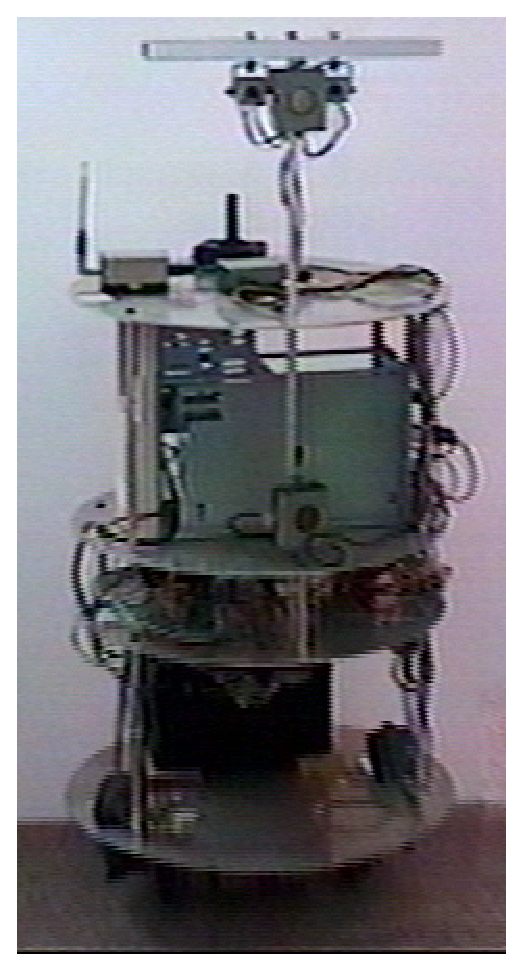
\includegraphics[width=0.65\linewidth]{Figures/twil6.ps}
	\caption{The Twil Mobile Robot.}
	\label{fig:twil}
\end{center}
\end{figure}

\section{Conclusion}
\label{sec:conclusions}

This paper presented an application of MPC to a nonholonomic WMR. The solution of the optimization problem through a standard QP method was shown. The obtained control signals were such that the constraints imposed on the control variables were respected. Real time experiments are undergoing and their results should be available for the final version of this paper.

\section{Acknowledgments}

The authors gratefully acknowledge the financial support from CAPES.

\bibliographystyle{IEEEtran}
\bibliography{mechrob04_v6}

\end{document}


